\Underline{Note!} In this case we have
\[\Braket{\Creab_{\v{q}}\Annib_{\v{q}}}\neq\dfrac{1}{e^{\beta\omega_{\v{q}}}-1}.\]
Instead we find, using equation~\eqref{eq:n_a}:
\[\Braket{\Creab_{\v{q}}\Annib_{\v{q}}}=v_{\v{q}}^2+\left(u_{\v{q}}^2+v_{\v{q}}^2\right)\dfrac{1}{e^{\beta\omega_{\v{q}}}-1}.\]
This means that we can write $\Ma_\text{A}$ as
\[\Ma_\text{A}=N_\text{A}S-\Sum_{\v{q}}\left[v_{\v{q}}^2+\left(u_{\v{q}}^2+v_{\v{q}}^2\right)\dfrac{1}{e^{\beta\omega_{\v{q}}}-1}\right].\]
\textcolor{red!80!black}{\emph{(...) dependent correction (...),}}
\[\tanh(2\theta)=\dfrac{2\gamma_{\v{q}}}{z}=\dfrac{2\tanh(\theta)}{1+\tanh^2(\theta)},\]
where $z=2d$ on a \Underline{cubic} $d$-dimensional lattice.
\[\tilde{\gamma}_{\v{q}}\equiv\dfrac{2\gamma_{\v{q}}}{z}=\dfrac{1}{d}\Sum_{\alpha=1}^d\cos(q_\alpha),\]
or by defining
\[t\equiv\tanh(\theta),\qquad s\equiv\sinh(\theta),\qquad c\equiv\cosh(\theta),\]
\[\tilde{\gamma}_{\v{q}}=\dfrac{2t}{1+t^2}\qquad\Rightarrow\qquad\tilde{\gamma}_{\v{q}}^2=\dfrac{4t^2}{(1+t^2)^2}=\dfrac{4s^2c^2}{(c^2+s^2)^2}.\]
Remember: $c^2-s^2=1$, which means that
\[\tilde{\gamma}_{\v{q}}^2=4\dfrac{s^2(1+s^2)}{(1+2s^2)^2}.\]
We now introduce $x\equiv s^2$ and $b\equiv\tilde{\gamma}_{\v{q}}^2/4$:
\[b=\dfrac{x(1+x)}{(1+2x)^2}\qquad\xRightarrow{\;x>0\;}\qquad x=-\dfrac{1}{2}+\dfrac{1}{2}\,\dfrac{1}{\sqrt{1-4b}}.\]
This means that we find
\[\sinh^2(\theta)=v_{\v{q}}^2=\dfrac{1}{2}\left(\dfrac{1}{\sqrt{1-\tilde{\gamma}_{\v{q}}^2}}-1\right),\qquad u_{\v{q}}^2=1+v_{\v{q}}^2=\dfrac{1}{2}\left(\dfrac{1}{\sqrt{1-\tilde{\gamma}_{\v{q}}^2}}+1\right).\]
Combining these results:
\[\boxed{u_{\v{q}}^2+v_{\v{q}}^2=\dfrac{1}{\sqrt{1-\tilde{\gamma}_{\v{q}}^2}}.}\]
As was shown in assignment 3,
\[\omega_q=4|J|Sd\left(1-\tilde{\gamma}_{\v{q}}^2\right)^2.\]
For a $d$-dimensional ``cubic'' lattice we can write
\[\begin{array}{r@{\;}c@{\;}l}
	\tilde{\gamma}_{\v{q}}							& =			& \dfrac{1}{d}\left(d-\dfrac{\v{q}^2}{2}+\cdots\right)=1-\dfrac{\v{q}^2}{2d}+\cdots,\\\\
	\tilde{\gamma}_{\v{q}}^2						& \approx	& 1-\dfrac{\v{q}^2}{d}+\cdots,\\\\
	1-\tilde{\gamma}_{\v{q}}^2						& =			& \dfrac{\v{q}^2}{d}+\cdots,\\\\
	\dfrac{1}{\sqrt{1-\tilde{\gamma}_{\v{q}}^2}}	& =			& \dfrac{\sqrt{d}}{|\v{q}|}+\cdots=u_{\v{q}}^2+v_{\v{q}}^2.\qquad(|\v{q}|\ll1.)
\end{array}\]
Substituting this back, we get
\[\omega_{\v{q}}=4|J|S\sqrt{d}|\v{q}|\]
when $|\v{q}|\ll1$, which in the case of $d=2$ is in agreement with equation~\eqref{eq:omega_ferromagnetic}. The temperature-dependent correction to the magnetization can now be calculated:
\begin{equation}\label{eq:delta_ma_integral}\begin{array}{r@{\;}c@{\;}l}
	\Delta\Ma(T)	& =			& -\Sum_{\v{q}}\left(u_{\v{q}}^2+v_{\v{q}}^2\right)\dfrac{1}{e^{\beta\omega_{\v{q}}}-1}\\\\
					& \approx	& -\Sum_{\v{q}}\dfrac{\sqrt{d}}{|\v{q}|}\dfrac{1}{e^{\beta|J|\eta|\v{q}|}-1}\qquad\text{(Low T.)}\\\\
					& =			& -\beta\Omega_d\Int_0^\infty d|\v{q}|\,\dfrac{|\v{q}|^{d-2}}{e^{\beta|J|\eta|\v{q}|}-1}.
\end{array}\end{equation}
Making a change of variables by introducing
\[x=\beta|J|\eta|\v{q}|,\]
the integral is evaluated as
\[\Delta\Ma(T)\propto\left(\dfrac{1}{\beta|J|\eta}\right)^{d-2+1}\Int_0^\infty dx\,\dfrac{x^{d-2}}{e^x-1}\propto\left(\dfrac{T}{|J|}\right)^{d-1}.\]
In the case where $d=3$ this means that
\[\Delta\Ma(T)\propto\left(\dfrac{T}{|J|}\right)^2\qquad\text{(\Underline{Antiferromagnetic})}.\]
Recall the ferromagnetic case, in which for $d=3$ we got (\textcolor{red!80!black}{equation reference needed})
\[\Delta\Ma(T)\propto\left(\dfrac{T}{|J|}\right)^{3/2}.\]
Comparing the two, we can say that
\begin{figure}
	\centering
	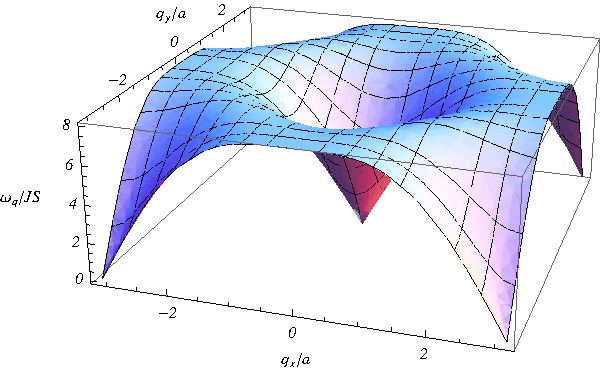
\includegraphics{img/omega_antiferromagnetic_compress}
	\caption{\label{fig:omega_antiferromagnetic_compress}The angular frequency $\omega_{\B{q}}$ as a function of the momentum $\B{q}$ for the antiferromagnetic case described by equation~\eqref{eq:omega_antiferromagnetic}.}
\end{figure}
\[\Delta\Ma_{\text{AF}}(T)=\Delta\Ma_{\text{Ferro}}(T)\cdot\left(\dfrac{T}{|J|}\right)^{1/2}\ll\Delta\Ma_{\text{Ferro}}(T).\qquad(T/J\ll1.)\]
The corrections to $\Ma$ due to \Underline{temperature effects} are weaker in antiferromagnets than in ferromagnets. This can be seen from the magnon spectrum (compare figures~\ref{fig:omega_ferromagnetic_compress} and~\ref{fig:omega_antiferromagnetic_compress}). It is \Underline{easier} to thermically excite ferromagnetic magnons than antiferromagnetic ones. We thus find a bigger temperature correction for the magnetization in a ferromagnet than in an antiferromagnet.

\Underline{But!} Note that ferromagnets don't have quantum fluctuations, while antiferromagnets do.

There are fluctuations even at zero temperature:
\[\Sum_{\v{q}}v_{\v{q}}^2=\dfrac{1}{2}\Sum_{\v{q}}\left(\dfrac{1}{\sqrt{1-\tilde{\gamma}_{\v{q}}^2}}-1\right)=\dfrac{\sqrt{d}}{2}\Sum_{\v{q}}\dfrac{1}{|\v{q}|}-\left(\dfrac{N_{\text{A}}}{2}\right),\]
which for $T=0$ gives
\[\Ma_{\text{A}}=N_{\text{A}}\left(S+\dfrac{1}{2}\right)-\Sum_{\v{q}}\dfrac{\sqrt{d}}{2}\dfrac{1}{|\v{q}|}.\]
For large $|\v{q}|$ \textcolor{red!80!black}{(Brillouin zone)} no problem with \textcolor{red!80!black}{integers}. For small $|\v{q}|$ the integral in equation~\eqref{eq:delta_ma_integral} becomes
\[\Omega_d\Int dq\,q^{d-2},\]
which for $d=2$ is ok for small $|\v{q}|$, but for $d=1$ we get
\[\Int_{1/L}^1dq\,\dfrac{1}{q}\propto\ln L,\]
a divergent function with weak divergence when $L\rightarrow\infty$. For $T=0$ the quantum fluctuations are large when $d=1$.

As can be seen from figure~\ref{fig:neel_state_sublattice} the corners of the Brillouin zone are not involved. \textcolor{red!80!black}{This is why} only small $|\v{q}|$ contribute.




\subsection{Quantization of lattice vibrations: phonons}
First look at a 1D lattice model (only look at the ion vibrations). The Hamiltonian for such a lattice system has the classical form
\[\Ha=\Sum_{i}\Sum{\v{P}_i^2}{2M}+\Sum_{n=1}^N\Sum_{m=1}^{\#\text{ neighbours}}V(R_n-R_{n+m}).\]
Here $V(x)$ is a microscopic pair potential that works between the ions. This is not limited to nearest-neighbour interaction. We can write
\[R_n=R_n^0+x_n,\]
with $R_n$ for the equilibrium position of lattice point $n$ and $x_n$ for the small deviation from it. For small fluctuations around the equilibrium position, the lattice will exhibit \Underline{harmonic} oscillations.

Taylor expanding $V(R_n-R_{n+m})$ to second order, we find
\[\begin{split}\Sum_{n,m}V(R_n-R_{n+m})=&\underbrace{\Sum_{n,m}V(R_n^0-R_{n+m}^0)}_{\text{constant}}+\underbrace{\left.\Sum_{n,m}\dfrac{\partial V}{\partial x}\right|_{x=R_n^0-R_{n+m}^0}(x_n-x_{n+m})}_{=0\text{ since we expand around a minimum}}\\[0.5\baselineskip]&+\dfrac{1}{2}\left.\Sum_{n,m}\dfrac{\partial^2V}{\partial x^2}\right|_{x=R_n^0-R_{n+m}^0}(x_n-x_{n+m})^2+\cdots\end{split}\]
Defining now
\[\Phi(R_n^0-R_{n+m}^0)\equiv\left.\dfrac{\partial^2V}{\partial x^2}\right|_{x=R_n^0-R_{n+m}^0}>0,\]
the significant term becomes
\[\dfrac{1}{2}\Sum_{n,m}\Phi(R_n^0-R_{n+m}^0)(x_n^2+x_{n+m}^2-2x_nx_{n+m}).\]
Since
\[\Phi(R_n^0-R_{n+m}^0)=\Phi(R_m^0)\]
and
\[\left.\begin{array}{r@{\;}c@{\;}l}
	R_n^0	& =	& an\\\\
	R_{n+m}	& =	& a(n+m)
\end{array}\right\}\quad\Rightarrow\quad R_n^0-R_{n+m}^0=-R_m^0,\]
we find
\[\Phi(x)=\Phi(-x),\]
with which we get
\[\Sum_{n,m}V(R_n^0-R_{n+m}^0)=\dfrac{1}{2}\Sum_m\Phi(R_m^0)\Sum_n\left(x_n^2+x_{n+m}^2-2x_nx_{n+m}\right).\]
We wish to write this in the form of harmonic oscillations, to which end we introduce new variables that ``decouple'' the potential term. This will be done, as we did in assignment 2, exercise 1, with Fourier-transformed variables:
\[x_n=\dfrac{1}{\sqrt{N}}\Sum_k\tilde{x}_k\,e^{ikn},\qquad\tilde{x}_k=\dfrac{1}{\sqrt{N}}\Sum_nx_n\,e^{-ikn}.\]
With this we get:
\[\Sum_nx_nx_{n+m}=\Sum_k\tilde{x}_k\tilde{x}_{-k}\,e^{-ikn},\]
which means that the potential term becomes
\[\Sum_{n,m}V(R_n-R_{n+m})=\Sum_k\underbrace{\left(\Sum_{m\in\text{neighbours}}\Phi(R_m^0)\left[1-\cos(km)\right]\right)}_{\equiv{\dfrac{1}{2}\omega_k^2M}}\tilde{x}_k\tilde{x}_{-k}.\]
We can also Fourier transform the momentum:
\[\begin{array}{r@{\;}c@{\;}l}
	p_n						& =	& \dfrac{1}{\sqrt{N}}\Sum_k\tilde{p}_k\,e^{-ikn},\\\\
	\tilde{p}_k				& =	& \dfrac{1}{\sqrt{N}}\Sum_np_n\,e^{ikn},\\\\
	\Sum_n\dfrac{p_n^2}{2M}	& =	& \Sum_k\dfrac{\tilde{p}_k\tilde{p}_{-k}}{2M}.
\end{array}\]
The Hamiltonian for a one-dimensional lattice, in the harmonic approximation, then becomes:
\[\boxed{\Ha=\Sum_k\left(\dfrac{\tilde{p}_k\tilde{p}_{-k}}{2M}+\dfrac{M\omega_k^2}{2}\,\tilde{x}_k\tilde{x}_{-k}\right).}\]
This is the standard form of a harmonic oscillator, the sum of 1D harmonic, \Underline{independent} oscillators. We will second quantize this by introducing creation and annihilation operators exactly as for a single 1D harmonic oscillator, for each $k$ value.
\[\begin{array}{r@{\;}c@{\;}l}
	\tilde{x}_k							& =	& \sqrt{\dfrac{\hbar}{2m\omega_k}}\left(\Creab_{-k}+\Annib_k\right)\\\\
	\tilde{p}_k							& =	& i\sqrt{\dfrac{m\omega_k\hbar}{2}}\left(\Creab_k-\Annib_{-k}\right),\\\\
	\commum{\Annib_k,\Creab_{k'}}		& =	& \delta_{k,k'},\\\\
	\commum{\tilde{x}_k,\tilde{p}_{k'}}	& =	& i\hbar\delta_{k,k'},\\\\
	\commum{x_n,p_{n'}}					& =	& i\hbar\delta_{n,n'}.
\end{array}\]
Substituting back into the Hamiltonian,
\[\boxed{\Ha=\Sum_k\hbar\omega_k\left(\Creab_k\Annib_k+\dfrac{1}{2}\right),}\]
as one would have guessed. The last term is a ``zero point'' energy, which we will drop hereafter. The (harmonic) lattice vibrations will we quantized to a \Underline{free boson gas}. The quantized excitations of the sound field are called \Underline{phonons}, and have creation/annihilation operators $\Creab_k$, $\Annib_k$. This is entirely analogous to the quantized excitations of spin waves, which we called magnons.

\subsection{Non-harmonics}
The series expansion of
\[\Sum_{n,m}V(R_n-R_{n+m})\]
to higher order than \Underline{quadratic} gives non-harmonic fluctuations. We will look at the third order term, which gives the first corrections to the ideal boson gas picture.
\[\dfrac{1}{3!}\Sum_{n,m}\underbrace{\left.\dfrac{\partial^3V}{\partial x^3}\right|_{x=R_n^0-R_{n+m}^0}}_{\Gamma(R_n^0-R_{n+m}^0)=\Gamma(R_{m}^0)}(x_n-x_{n+m})^3=\dfrac{1}{6}\Sum_m\Gamma(R_m^0)\Sum_n(x_n-x_{n+m})^3.\]
We again introduce the Fourier modes to the fluctuations:
\[\begin{array}{r@{\;}c@{\;}l}
	\Sum_nx_n^3	& =	& \Sum_n\left(\dfrac{1}{\sqrt{N}}\Sum_{k_1}\tilde{x}_{k_1}\,e^{ik_1n}\right)\left(\dfrac{1}{\sqrt{N}}\Sum_{k_2}\tilde{x}_{k_2}\,e^{ik_2n}\right)\left(\dfrac{1}{\sqrt{N}}\Sum_{k_3}\tilde{x}_{k_3}\,e^{ik_3n}\right)\\\\
				& =	& \dfrac{1}{\sqrt{N}}\Sum_{k_{1,2,3}}\tilde{x}_{k_1}\tilde{x}_{k_2}\tilde{x}_{k_3}\underbrace{\dfrac{1}{N}\Sum_ne^{i(k_1+k_2+k_3)n}}_{\delta_{k_1-k_2-k_3}}\\\\
				& =	& \boxed{\dfrac{1}{\sqrt{N}}\Sum_{k_1,k_2}\tilde{x}_{k_1}\tilde{x}_{k_2}\tilde{x}_{-k_1-k_2}}
\end{array}\]